 
\begin{center}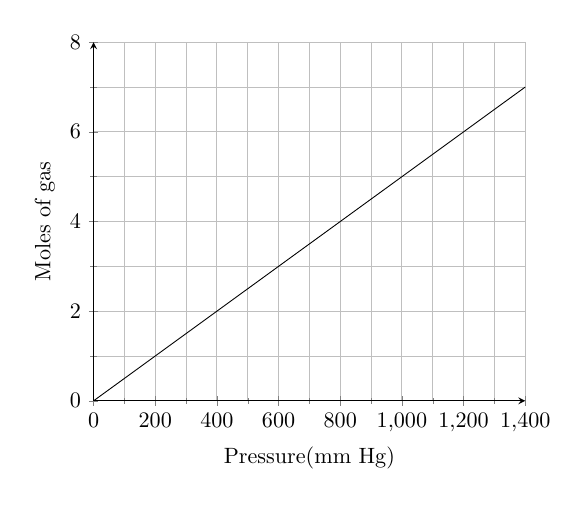
\begin{tikzpicture}[scale=0.8]\begin{axis}[axis lines=left, ylabel=Moles of gas, xlabel=Pressure(mm Hg),grid=both, xmin=0, xmax=1400, ymin=0, ymax=8,minor tick num=1, ]
\addplot[domain=0:1400,samples=3,]{x/200};
\end{axis}\end{tikzpicture}\end{center}
A particular sample of gas behaves in accordance with ideal gas principles under its controlled volume and temperature.  Which of the following functions most accurately predicts the pressure ($P$) of the gas sample given the sample's moles ($M$) for a point on this graph?


\ifsat
	\begin{enumerate}[label=\Alph*)]
		\item $P=$ {\Large$\frac{1}{200}$} $M$
		\item $P-3=200(M-600)$
		\item $P-600=$ {\Large$\frac{1}{200}$} $(M-3)$
		\item $P-600=200(M-3)$ % 
	\end{enumerate}
\else
\fi

\ifacteven
	\begin{enumerate}[label=\textbf{\Alph*.},itemsep=\fill,align=left]
		\setcounter{enumii}{5}
		\item $P=$ {\Large$\frac{1}{200}$} $M$
		\item $P-3=200(M-600)$
		\item $P-600=$ {\Large$\frac{1}{200}$} $(M-3)$
		\addtocounter{enumii}{1}
		\item $P-600=200(M-3)$ % 
		\item $P-3=$ {\Large$\frac{1}{200}$} $(M-600) $
	\end{enumerate}
\else
\fi

\ifactodd
	\begin{enumerate}[label=\textbf{\Alph*.},itemsep=\fill,align=left]
		\item $P=$ {\Large$\frac{1}{200}$} $M$
		\item $P-3=200(M-600)$
		\item $P-600=$ {\Large$\frac{1}{200}$} $(M-3)$
		\item $P-600=200(M-3)$ % 
		\item $P-3=$ {\Large$\frac{1}{200}$} $(M-600) $
	\end{enumerate}
\else
\fi

\ifgridin
 $P-600=200(M-3)$ % 

\else
\fi

